\begin{figure*}[!htbp]
\centering
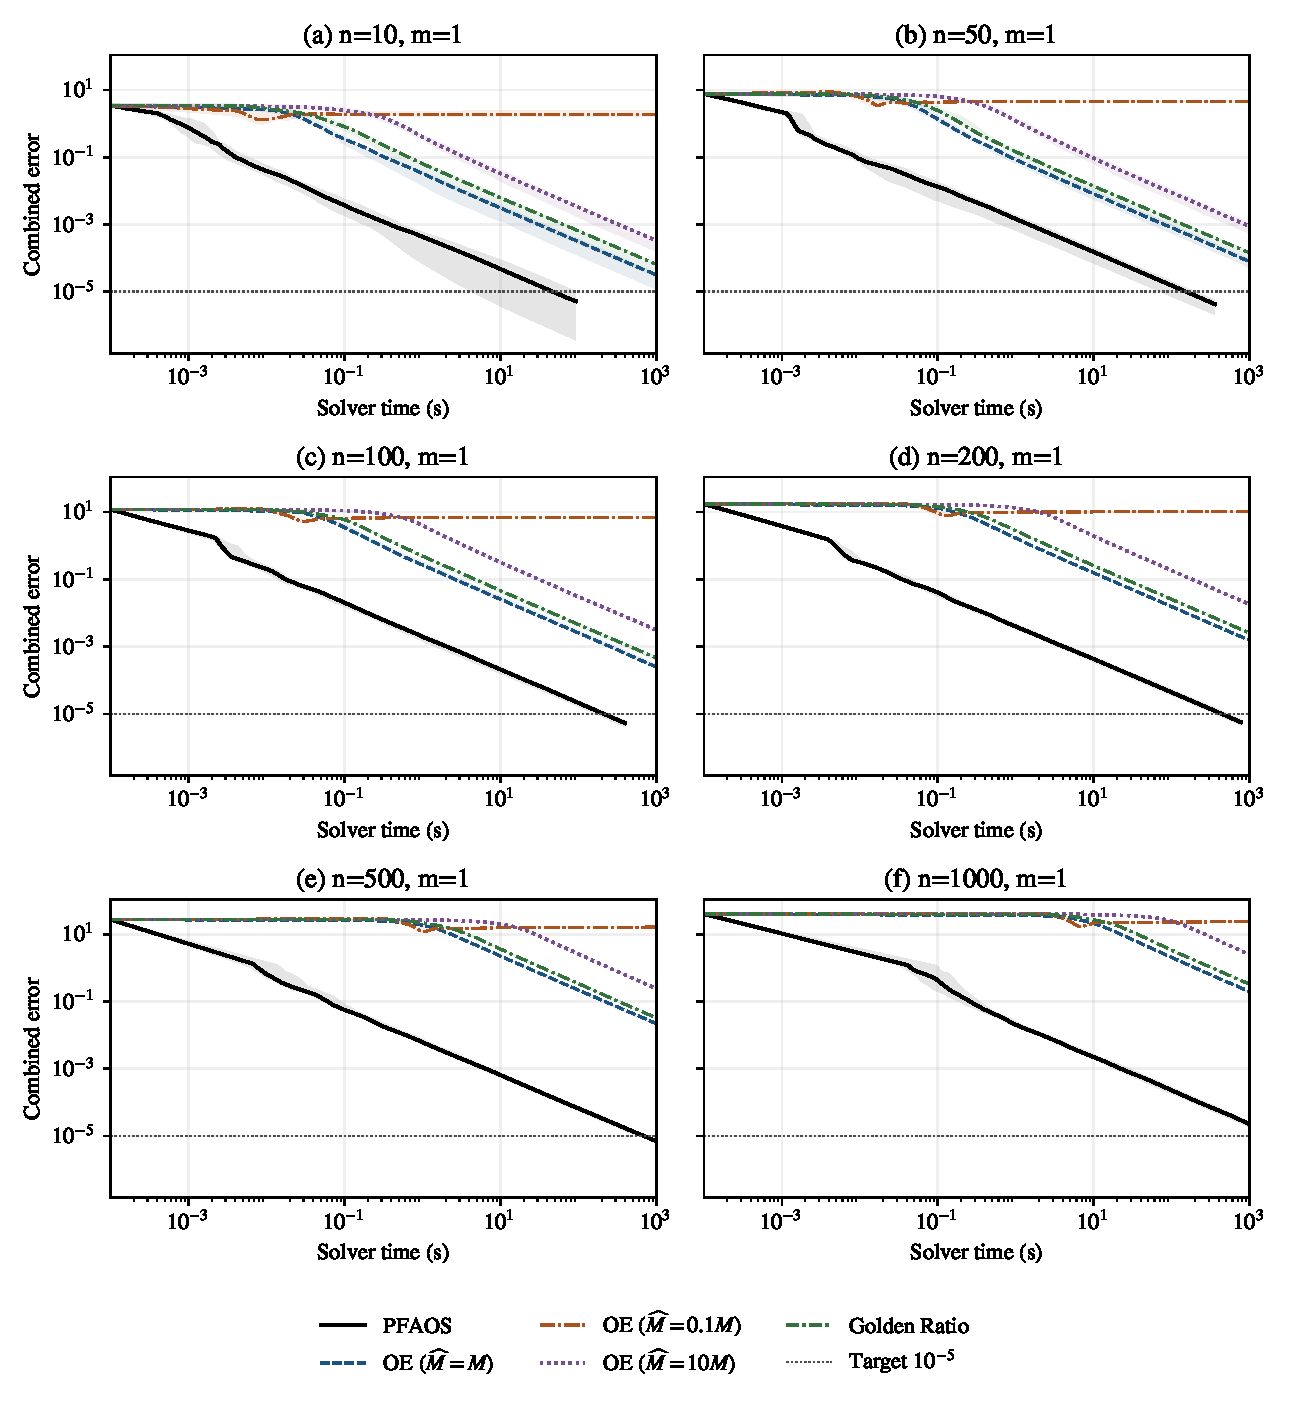
\includegraphics[width=\textwidth]{pfaos_full_grid.pdf}
\caption{Combined numerical error over the single-constraint grid ($m=1$; $n=10$, $n=50$, $n=100$, $n=200$, $n=500$, $n=1000$). Curves are medians over 10 seeds, with pointwise 95\% bootstrap confidence intervals for each median. Each method uses a fixed complete seed set and ends at the earliest observed terminal checkpoint. Aggregation requires at least two saved points and complete valid gap coverage for every seed; unavailable methods are explicitly identified. Log--log interpolation and a $10^{-12}$ display floor are for visualization only; tables use unmodified values and saved checkpoint times. The dotted line is $10^{-5}$. Later per-seed attainments may lie beyond the common aggregate horizon.}
\label{fig:pfaos_full_grid}
\end{figure*}
